\documentclass{sigchi-ext}
% Please be sure that you have the dependencies (i.e., additional
% LaTeX packages) to compile this example.
\usepackage[T1]{fontenc}
\usepackage{textcomp}
\usepackage[scaled=.92]{helvet} % for proper fonts
%\usepackage{graphicx} % for EPS use the graphics package instead
\usepackage{epsfig} % Max added
\usepackage{tabularx} % Max added
\usepackage{balance}  % for useful for balancing the last columns
\usepackage{booktabs} % for pretty table rules
\usepackage{ccicons}  % for Creative Commons citation icons
\usepackage{ragged2e} % for tighter hyphenation

% Some optional stuff you might like/need.
% \usepackage{marginnote}
% \usepackage[shortlabels]{enumitem}
% \usepackage{paralist}
% \usepackage[utf8]{inputenc} % for a UTF8 editor only

%% EXAMPLE BEGIN -- HOW TO OVERRIDE THE DEFAULT COPYRIGHT STRIP --
% \copyrightinfo{Permission to make digital or hard copies of all or
% part of this work for personal or classroom use is granted without
% fee provided that copies are not made or distributed for profit or
% commercial advantage and that copies bear this notice and the full
% citation on the first page. Copyrights for components of this work
% owned by others than ACM must be honored. Abstracting with credit is
% permitted. To copy otherwise, or republish, to post on servers or to
% redistribute to lists, requires prior specific permission and/or a
% fee. Request permissions from permissions@acm.org.\\
% {\emph{CHI'14}}, April 26--May 1, 2014, Toronto, Canada. \\
% Copyright \copyright~2014 ACM ISBN/14/04...\$15.00. \\
% DOI string from ACM form confirmation}
%% EXAMPLE END

% Paper metadata (use plain text, for PDF inclusion and later
% re-using, if desired).  Use \emtpyauthor when submitting for review
% so you remain anonymous.
\def\plaintitle{One-Step, Three-Factor Authentication in a Single Earpiece} \def\plainauthor{Max T. Curran, Nick Merrill, Swapan Gandhi, and John Chuang}
%\def\emptyauthor{}
\def\plainkeywords{multifactor authentication; passthoughts, usable security}
%\def\plaingeneralterms{Documentation, Standardization}

\title{One-Step, Three-Factor Authentication in a Single Earpiece}

\numberofauthors{4}
% Notice how author names are alternately typesetted to appear ordered
% in 2-column format; i.e., the first 4 autors on the first column and
% the other 4 auhors on the second column. Actually, it's up to you to
% strictly adhere to this author notation.

\author{
  \alignauthor{
    \textbf{Max T. Curran}\\
    \affaddr{BioSENSE Lab}\\
    \affaddr{School of Information}\\
    \affaddr{University of California, Berkeley}\\
    \affaddr{Berkeley, CA 94720, USA}\\
    \email{mtcurran@ischool.berkeley.edu}
  }\alignauthor{
    \textbf{Swapan Gandhi}\\
    \affaddr{Starkey Hearing Resaerch Center}\\
    \affaddr{Berkeley, CA 94724, USA}\\
    \email{Swapan\_Gandhi@starkey.com}
  }\vfil
  \alignauthor{
    \textbf{Nick Merrill}\\
    \affaddr{BioSENSE Lab}\\
    \affaddr{School of Information}\\
    \affaddr{University of California, Berkeley}\\
    \affaddr{Berkeley, CA 94720, USA}\\
    \email{ffff@berkeley.edu}
  }\alignauthor{
    \textbf{John Chuang}\\
    \affaddr{BioSENSE Lab}\\
    \affaddr{School of Information}\\
    \affaddr{University of California, Berkeley}\\
    \affaddr{Berkeley, CA 94720, USA}\\
    \email{chuang@ischool.berkeley.edu}
  }
}

% Make sure hyperref comes last of your loaded packages, to give it a
% fighting chance of not being over-written, since its job is to
% redefine many LaTeX commands.
\definecolor{linkColor}{RGB}{6,125,233}
\hypersetup{%
  pdftitle={\plaintitle},
  pdfauthor={\plainauthor},
 % pdfauthor={\emptyauthor},
  pdfkeywords={\plainkeywords},
  bookmarksnumbered,
  pdfstartview={FitH},
  colorlinks,
  citecolor=black,
  filecolor=black,
  linkcolor=black,
  urlcolor=linkColor,
  breaklinks=true,
}

%\reversemarginpar%

\begin{document}

%% For the camera ready, use the commands provided by the ACM in the Permission Release Form.
%\CopyrightYear{2007}
%\setcopyright{rightsretained}
%\conferenceinfo{WOODSTOCK}{'97 El Paso, Texas USA}
%\isbn{0-12345-67-8/90/01}
%\doi{http://dx.doi.org/10.1145/2858036.2858119}
%% Then override the default copyright message with the \acmcopyright command.
%\copyrightinfo{\acmcopyright}

\maketitle

% Uncomment to disable hyphenation (not recommended)
% https://twitter.com/anjirokhan/status/546046683331973120
\RaggedRight{} 

% Do not change the page size or page settings.
\begin{abstract}
 Multifactor authentication presents a robust method to secure our digital private information, but typically requires multiple actions on the part of the user resulting in a high cost to usability and limiting adoption. Furthermore, a truly usable system must be unobtrusive and inconspicuous. Here, we present a system that provides all three factors of authentication (knowledge, possession, and inherence) in a single step in the form of an earpiece which implements brain-based authentication via custom-fit, in-ear electroencephalography (EEG). We demonstrate its potential by collecting electroencephalography (EEG) data using manufactured custom-fit earpieces with embedded electrodes. Across 7 participants, we are able to achieve perfect performance, mean 0\% false acceptance (FAR) and 0\% false rejection rates (FRR), using participants' best performing tasks with data from only one earpiece with three electrodes. Our results indicate that a single earpiece with embedded electrodes could provide a discreet, convenient, and robust method for secure one-step, three-factor authentication.
\end{abstract}

\keywords{\plainkeywords}

\category{H.5.m}{Information interfaces and presentation (e.g.,
  HCI)}{Miscellaneous}

  %\category{See}{\url{http://acm.org/about/class/1998/}}{for
  %full list of ACM classifiers. This section is required.}

\section{Introduction}
It is well appreciated by experts and end-users alike that strong authentication is
critical to cybersecurity and privacy, now and into the future. Unfortunately,
news reports of celebrity account hackings serve as regular reminders that
the currently dominant method of authentication in consumer applications, 
single-factor authentication using passwords or other user-chosen secrets, 
faces many challenges. Major industry players such as Google and
Facebook have strongly encouraged their users to adopt two-factor
authentication (2FA). However, submitting authenticators in two separate steps
 has frustrated wide adoption due to its additional hassle to users. In this study we undertake, to the best of our knowledge, the first ever exploration of one-step, three-factor authentication. In computer security,
authenticators are classified into three types: knowledge factors (e.g., passwords
and PINs), possession factors (e.g., physical tokens, ATM cards), and inherence
factors (e.g., fingerprints and other biometrics). By taking advantage of a physical token 
in the form of personalized earpieces, the uniqueness of an individual's brainwaves, and
a choice of mental task to use as one's "passthought", we seek to achieve all three factors 
of authentication in a single step by the user. Furthermore, the form factor of an earpiece carries significantly less stigma versus scalp-based passthoughts systems. Technology worn in the ear is already an acceptable practice, for example earphones or bluetooth headsets.

% \section{ACM Copyrights \& Permission}
% Accepted extended abstracts and papers will be distributed in the
% Conference Publications. They will also be placed in the ACM Digital
% Library, where they will remain accessible to thousands of researchers
% and practitioners worldwide. To view the ACM's copyright and
% permissions policy, see:
% \url{http://www.acm.org/publications/policies/copyright_policy}.

\section{Related Work}
The use of EEG as a biometric signal for user authentication has a relatively short history.
In 2005, Thorpe et al. motivated and outlined the design of a passthoughts system \cite{Thorpe2005}.
Since 2002, a number of independent groups have achieved 99-100\% authentication accuracy for small populations using research-grade and consumer-grade scalp-based EEG systems \cite{Poulos2002,Marcel2007a,Ashby2011,Chuang2013b}.

The concept of in-ear EEG was introduced in 2011 with a demonstration of the feasibility of recording brainwave signals from within the ear canal \cite{Looney2011}. The in-ear placement can produce signal-to-noise ratios comparable to those from conventional EEG electrode placements, is robust to common sources of artifacts, and can be used in a brain-computer interface (BCI) system based on auditory and visual evoked potentials \cite{Kidmose2013a}. An 80\% accuracy level was achieved for user authentication using in-ear EEG captured with a modified single-channel consumer-grade device \cite{curran2016passthoughts}.

Behavioral authentication methods such as keystroke dynamics and speaker authentication can be categorized as one-step two-factor authentication schemes. In both cases, the knowledge factor (password or passphrase) and inherence factor (typing rhythm or speaker's voice) are employed \cite{Monrose1997}. In contrast, the Nymi band supports one-step two-factor authentication via the inherence factor (cardiac rhythm that is supposed to be unique to each individual) and the possession factor (the wearing of the band on the wrist) \cite{Nymi}. However, as far as we know, no one has proposed or demonstrated a one-step three-factor authentication scheme.

% \subsection{Usable Authentication}

% When proposing or evaluating authentication paradigms robustness against imposters is often the first consideration, but the usability of these systems is of equal importance as they must conform to a person's needs and lifestyle to warrant adoption and prolonged use. The authors of \cite{sasse2001} describe usability issues with knowledge-based systems like alphanumeric passwords, in particular that it should not be the burden of the user to remember complex passwords that have to be frequently changed. \cite{braz2006} analyzed some of the complexities applying interface human factors heuristics to authentication, and indicate the importance of social acceptibility, learnability, and simplicity of authentication methods. Technology worn on the head faces particular usability issues; in their analysis of user perceptions of such devices, \cite{Genaro2014} identified design, usability, ease of use, and obtrusiveness among the top 10 concerns of users online postings, and qualitatively comments around comfort and "looking weird".

% In the proposed system we seek to incorporate the perspectives of HCI research on authentication. Passthoughts such as a favorite song or relaxed breathing are easy for a user to remember and perform, and the choice of an earpiece form factor of our system seeks to address wearability and social perception concerns.

% Mobile and wearable technologies' continuous proximity to the user's body provides favorable conditions for unobtrusively capturing biometrics for authentication. Many such uses have been proposed that embrace usability like touch-based interactions \cite{Tartz2015, Holz2015} and walking patterns \cite{Lu2014} using mobile phones, as well as identification via head movements and blinking in head-worn devices \cite{Rogers2015}. However, these typically draw only from the inherence factor. \cite{Chen2015} proposed an inherence and knowledge two-factor method for multi-touch mobile devices based on a user's unique finger tapping of a song, though it may be vulnerable to "shoulder surfing": imposters observing and mimicking the behavior. By comparison, passthoughts are largely invisible to attackers. Furthermore, this system also presents a possible solution to "rubber-hose attacks" (forceful coercion to divulge a password): a thought, which is secret (and thus changeable), but has a particular expression unique to an individual, the specific performance of which cannot be described (and thus cannot be coerced).

\begin{marginfigure}[-20pc]
\begin{minipage}{\marginparwidth}
  \centering
  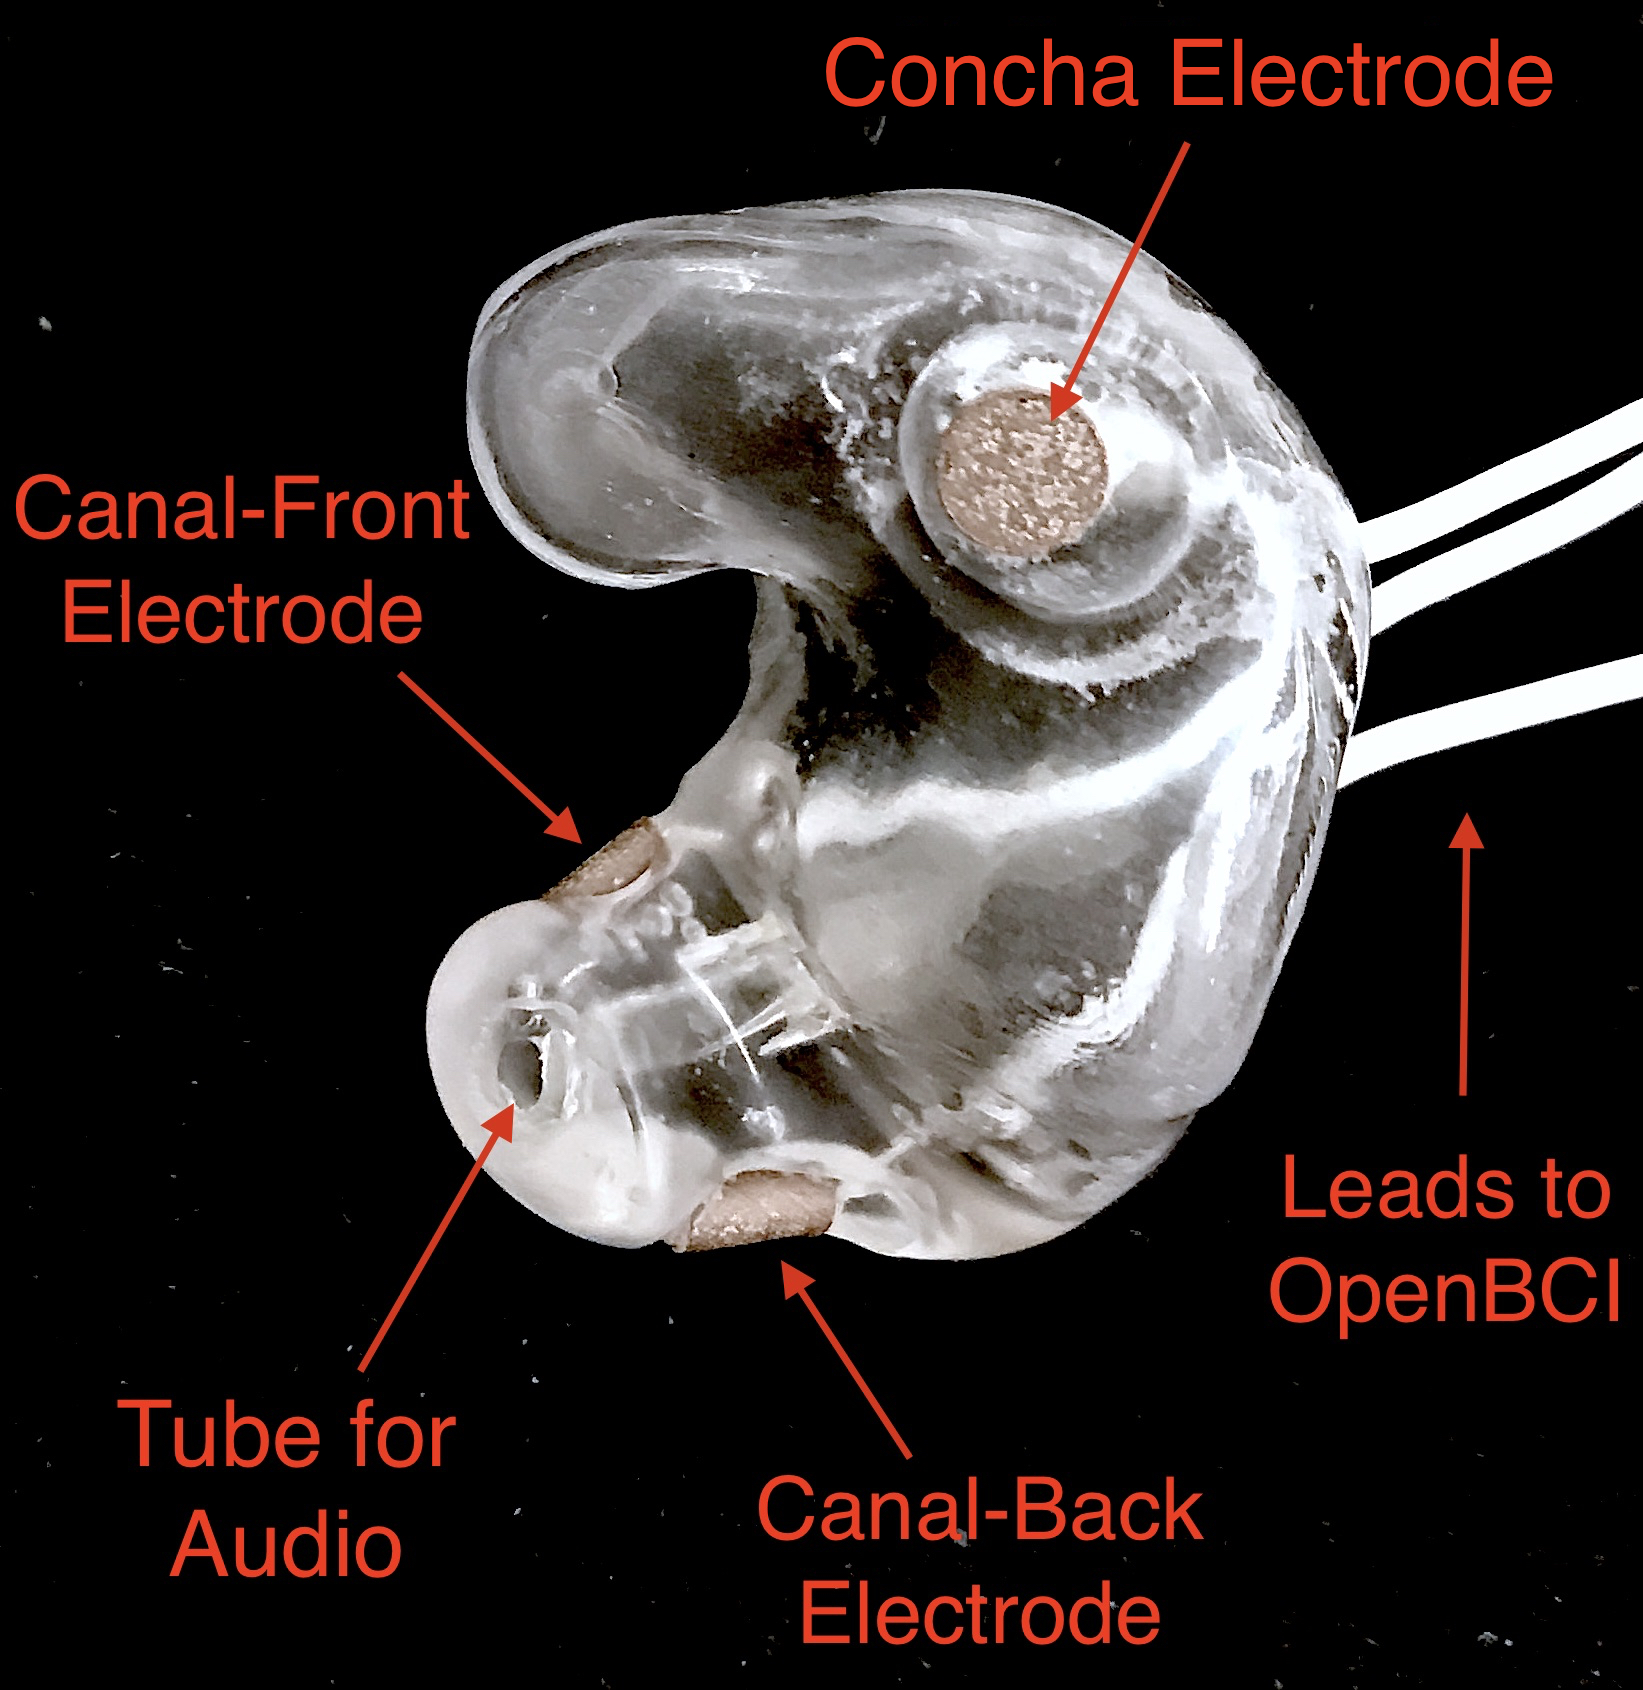
\includegraphics[width=0.9\marginparwidth]{figures/CFEEEG_piecefig_Right.jpg}
  \caption{Labeled photo of one of our manufactured custom-fit earpieces with 3 embedded electrodes located in the concha, front-facing (anterior) in the ear canal, and back-facing (posterior) in the ear canal.}\label{fig:earpiece_diagram}
\end{minipage}
\end{marginfigure}

\section{Methods}
To create the custom-fitted earpieces, a molding of each participant's ear was taken, 3D scanned, and the earpieces were manufactured with three AgCl electrodes installed in each, two in the ear canal and one at the concha, at positions simplified from those described in \cite{Mikkelsen2015}. One of the manufactured earpieces is shown in Figure \ref{fig:earpiece_diagram}.

We used an 8-channel OpenBCI system \cite{michalska2009openbci}, an open-source alternative to medical-grade EEG systems with demonstrated effectiveness \cite{Frey2016}. The ground was placed at the center of the forehead, approximately AFz according to the 10-20 International Standard for Electrode Placement (ISEP), and reference on the left mastoid. One AgCl ring electrode was placed at approximately Fp1 (ISEP location above the left eye) to validate the data collected in the ear against a common scalp-based placement. Before beginning the experiment, the data from each channel was visually inspected using the OpenBCI interface. Audio stimuli were delivered through small tubes in the earpieces. Stimuli were presented using PsychoPy \cite{peirce2007psychopy}. Participants performed a set of mental tasks we chose based on findings in related work regarding the relative strengths of different tasks in authentication accuracy and usability as reported by participants. \cite{Chuang2013b, curran2016passthoughts} Furthermore, given the in-ear placement of the electrodes and therefore the proximity to the temporal lobes containing the auditory cortex, we tested several novel authentication tasks based specifically on aural imagery or stimuli. Our strategy was to select tasks that captured a diversity across dimensions of external stimuli, involving a personal secret, eyes open or closed (due to known effects on EEG), and different types of mental imagery. All tasks were performed for five trials each, followed by another set of five trials each to reduce boredom and repetition effects. Each trial was 10 seconds in length, for a total of 10 trials or 100 seconds of data collected per task. Seven male participants (P1-P7) completed this study protocol approved by our local ethics review board.

\section{Analysis}
We validated data collected by the earpieces using the alpha-attentuation method. It is a well-known feature of EEG data that activity in the alpha-band (approx. 8-12 Hz) increases when the eyes are closed compared to when the eyes are open. We compared data from the \textit{breathe} task with that of the \textit{breathe - open} task.  This attenuation is clearly visible even in just a single trial's data from our earpieces and matches data seen in our Fp1 scalp electrode as shown in figure \ref{fig:alpha_atten}.

\begin{marginfigure}[5pc]
\begin{minipage}{0.95\marginparwidth}
  \centering
  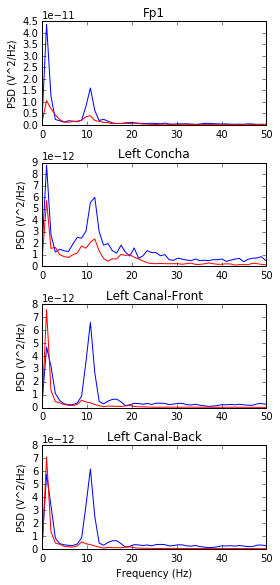
\includegraphics[width=0.9\marginparwidth]{figures/002_AlphaAtt_all.jpg}
  \caption{Alpha-attenuation (8-12 Hz range) in left ear and Fp1 channels, referenced at left mastoid. Red indicates breathing data with eyes open, blue indicates the same task with eyes closed.}\label{fig:alpha_atten}
\end{minipage}
\end{marginfigure}

We analyzed the EEG signals collected during the tasks using a support vector classifier (SVC). Since past work has shown that classification tasks in EEG-based brain-computer interfaces (BCI) are linear \cite{Garrett2003a}, we used XGBoost, a popular tool for logistic linear classification \cite{Chen2016}. To produce feature vectors, we took slices of 100 raw values from each electrode (about 500ms of data), and performed a fourier transform to produce power spectra for each electrode during that slice. We concatenated all electrode power spectra together, and performed principal component analysis on all concatenated vectors such that the resulting vectors described 95\% of the variance in the full power spectrum data. For each task, for each participant, 100 seconds of data were collected in total across 10 trials of 10 seconds each, resulting in 200 samples per participant, per task. We trained the classifier using a balanced sample of positive and negative examples, where positive examples were from the target participant and target task, and negative examples were randomly selected tasks from any participant besides the target participant. From this corpus of positive and negative samples, we withheld one third of data for testing. The remaining training set was fed into a XGBoost's cross-validation method and the updated classifier predicted labels on each sample in the test set. We calculated FAR and FRR from its results.

\begin{table*}
\centering
\begin{tabularx}{.85\textwidth}{lrrrrrrrrrr}
& \multicolumn{2}{c}{\textbf{P1}} & \multicolumn{2}{c}{\textbf{P2}} & \multicolumn{2}{c}{\textbf{P3}} & \multicolumn{2}{c}{\textbf{P5}} & \multicolumn{2}{c}{\textbf{P7}}\\
\textbf{Task} & FAR & FRR & FAR & FRR & FAR & FRR & FAR & FRR & FAR & FRR\\ \hline
Breathe & 0.0002 & 0 & 0 & 0 & 0 & 0 & 0 & 0.0127 & 0 & 0\\
Breathe - open & 0.0002 & 0.0127 & 0 & 0 & 0 & 0 & 0 & 0.0253 & 0 & 0\\
Face & 0.0002 & 0.0253 & 0.0005 & 0.0253 & 0 & 0.0127 & 0 & 0 & 0 & 0\\
Listen & 0 & 0 & 0.0005 & 0 & 0 & 0 & 0 & 0 & 0 & 0\\
Sequence & 0 & 0.0506 & 0.0002 & 0 & 0 & 0 & 0 & 0 & 0.0007 & 0.0127\\
Song   & 0.0002 & 0.0380 & 0 & 0 & 0 & 0 & 0 & 0.0127 & 0.0007 & 0.0127\\
Song - open & 0.0002 & 0.0127 & 0 & 0 & 0 & 0 & 0 & 0 & 0 & 0.0127\\
Speech & 0.0002 & 0 & 0.0005 & 0 & 0 & 0 & 0 & 0 & 0 & 0\\
Sport & 0.0002 & 0 & 0 & 0 & 0 & 0 & 0 & 0  & 0 & 0.0127\\ \hline
\textbf{Best Task} & \textbf{0} & \textbf{0} & \textbf{0} & \textbf{0} & \textbf{0} & \textbf{0} & \textbf{0} & \textbf{0} & \textbf{0} & \textbf{0}\\ \hline
\end{tabularx}
\caption{FAR and FRR performance of each task for each participant using data from the left ear. P4 and P6 achieve perfect zero FARs and FRRs across all tasks and so are not shown here.}
\label{tab:farfrrall}
\end{table*}

\begin{figure*}
\centering
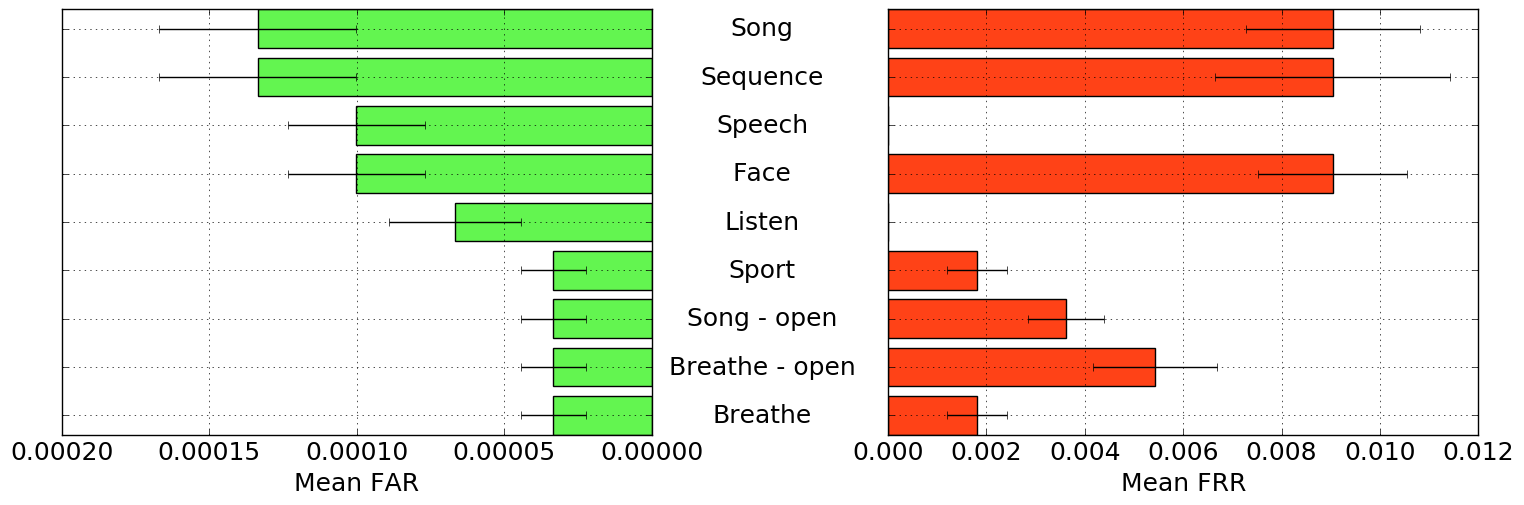
\includegraphics[width=.9\linewidth]{./figures/mean-far-and-frr-by-task.png}
\caption{FAR and FRR results by task, across all subjects, using data from the left ear only.}
\label{fig:meanByTask}
\end{figure*}

\section{Results}
The performance of each task for each participant is shown in Table \ref{tab:farfrrall}. For each participant we find at least one task for which they achieve 0\% FAR and FRR. We also calculated the mean FAR and FRR across all participants for each task, shown in Figure \ref{fig:meanByTask}.

\section{Discussion \& Limitations}
Our findings demonstrate the apparent feasibility of a passthoughts system consisting of a single earpiece with three electrodes and a reference, all on or around the left ear. FARs and FRRs are very low across all participants and tasks, with FARs overall lower than FRRs, a desirable pattern in terms of authenticating access to potentially sensitive information. Participants' best-performing passthoughts typically see no errors in our training. Several tasks performed exceedingly well among participants, even tasks like \textit{listen} and \textit{breathe} which didn't have an explicit secondary knowledge factor like in \textit{sport} or \textit{song}. This suggests a passthoughts system could present users with an array of options for them to choose from, though it remains to be seen how these tasks scale with larger populations.

The real-world implications of this study are limited by the small, relatively homogeneous sample of participants. In the case of this initial evaluation however, the homogeneity of our participant pool strengthens the reported results given that system is meant to distinguish between individuals. In order to establish the validity of this system for widespread real-world use we feel it is necessary to expand the size and diversity of participants in future work.

\section{Future Work}

% One primary question is how our passthoughts system performance will change with a greater number of users and with more diverse data. Our system specifically trains on negative examples of incorrect users; we do not yet know how this approach will scale. At the same time, we must investigate the stability of EEG readings for a passthought over time to establish long-term usability. We must also collect EEG data from the variety of different user states: ambulatory settings, during physical exertion or exercise, under the influence of caffeine or alcohol, etc.

% Another important question surrounds how passthoughts might be cracked. Generally, we do not understand how an individual's passthought is drawn from the distribution of EEG signals an individual produces throughout the day. Given a large enough corpus of EEG data, are some passthoughts as easy to guess as \textit{password1234} is for passwords? Future work should perform statistical analysis on passthoughts, such as clustering (perhaps with t-SNE) to better understand the space of possible passthoughts. This work will allow us simulate cracking attempts, and to develop empirically motivated strategies for prevention, e.g., locking users out after a certain number of attempts. This work could also reveal interesting tradeoffs between the usability or accuracy of passthoughts and their security.

Our work leaves room for some clear user experience improvements. Future work should assess dry electrodes, commonly found in consumer EEG devices, for comfort and usability. The electrodes could be grounded to the earlobe, instead of the forehead. Speakers could also be placed inside our current custom-fit earbuds to produce working "hearables" that could be used as ordinary headphones. Future work should also attempt a closed-loop (or online) passthought system, in which users receive immediate feedback on the result of their authentication attempt. A closed-loop BCI system would assist in understanding how human learning effects side might impact authentication performance, as the human and machine co-adapt.

\section{Conclusion}

As demonstrated by these preliminary results, custom-fit, in-ear EEG earpieces can provide three factors of security in one highly usable step: thinking one's passthought, using the discreet form factor of an earpiece. Among this initial sample, we are able to achieve 100\% authentication accuracy using a single sensing earpiece, showing potential for integration with technology already used in everyday life (like earphones). By expanding our corpus of EEG readings (in population size, time, and diversity of settings), we hope to better understand the underlying distribution of EEG signals and security properties of passthoughts as well usability issues that may arise in different contexts.

\section{Acknowledgments}
The authors would like to thank the Center for Long-Term Cybersecurity for funding this research.


% \begin{marginfigure}[-35pc]
%   \begin{minipage}{\marginparwidth}
%     \centering
%     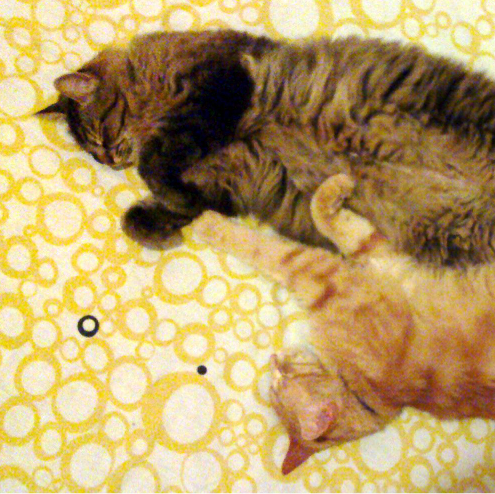
\includegraphics[width=0.9\marginparwidth]{figures/cats}
%     \caption{In this image, the cats are tessellated within a square
%       frame. Images should also have captions and be within the
%       boundaries of the sidebar on page~\pageref{sec:sidebar}. Photo:
%       \cczero~jofish on Flickr.}~\label{fig:marginfig}
%   \end{minipage}
% \end{marginfigure}

% \marginpar{\vspace{-23pc}So long as you don't type outside the right
%   margin or bleed into the gutter, it's okay to put annotations over
%   here on the left, too; this annotation is near Hawaii. You'll have
%   to manually align the margin paragraphs to your \LaTeX\ floats using
%   the \texttt{{\textbackslash}vspace{}} command.}

% \begin{margintable}[1pc]
%   \begin{minipage}{\marginparwidth}
%     \centering
%     \begin{tabular}{r r l}
%       & {\small \textbf{First}}
%       & {\small \textbf{Location}} \\
%       \toprule
%       Child & 22.5 & Melbourne \\
%       Adult & 22.0 & Bogot\'a \\
%       \midrule
%       Gene & 22.0 & Palo Alto \\
%       John & 34.5 & Minneapolis \\
%       \bottomrule
%     \end{tabular}
%     \caption{A simple narrow table in the left margin
%       space.}~\label{tab:table2}
%   \end{minipage}
% \end{margintable}

% \section{References Format}
% Your references should be published materials accessible to the
% public. Internal technical reports may be cited only if they are
% easily accessible and may be obtained by any reader for a nominal
% fee. Proprietary information may not be cited. Private communications
% should be acknowledged in the main text, not referenced (e.g.,
% [Golovchinsky, personal communication]). References must be the same
% font size as other body text. References should be in alphabetical
% order by last name of first author. Use a numbered list of references
% at the end of the article, ordered alphabetically by last name of
% first author, and referenced by numbers in brackets. For papers from
% conference proceedings, include the title of the paper and the name of
% the conference. Do not include the location of the conference or the
% exact date; do include the page numbers if available. 

\balance{} 

\bibliographystyle{SIGCHI-Reference-Format}
\bibliography{references}

\end{document}

%%% Local Variables:
%%% mode: latex
%%% TeX-master: t
%%% End:
